\chapter{相关理论与工作}
\section{引言}
本章从神经网络不确定性的建模方法、不确定性的计算,以及不确定性建模方法的评估三个方面,系统介绍神经网络不确定性的相关理论和研究工作。近年来,针对神经网络不确定性的建模方法层出不穷,包括基于单个神经网络的建模、集成多模型的建模,以及基于贝叶斯方法的神经网络建模,这些方法为不确定性的量化提供了多样化的理论基础和实现路径。

在不确定性的计算方面,研究主要集中于如何生成一个标量来量化神经网络的不确定性。部分方法将不确定性细分为数据不确定性和模型不确定性,分别进行建模;而另一些方法则直接对整体不确定性进行计算。

对于不确定性建模方法的评估,由于大多数情况下缺乏明确的不确定性标签,难以直接衡量方法的优劣。因此,通常通过代理任务(如分布外样本检测、对抗样本识别等)的表现,间接反映建模方法的有效性和性能。

以下将从上述三个方面逐一展开论述。


\section{不确定性的建模方法}
目前,在建模神经网络不确定性的方向上,相关研究提出了许多不同的方法:
\begin{itemize}
    \item 贝叶斯神经网络:通过在神经网络中引入贝叶斯推断,建模权重参数的不确定性,从而获得模型的输出不确定性。
    \item 模型集成的方法:通过训练多个神经网络,对于同一个输入,可以得到多个预测结果,进而通过计算多个预测值的方差或者熵来建模不确定性
    \item 测试时增强的方法:通过对输入做数据增强,得到多个增强后的输入,然后进入训练好的神经网络中预测多次得到多个预测结果,进而计算模型输出的不确定性。
    \item 单一确定的神经网络来建模不确定性:这类方法使用单一确定性的神经网络直接建模不确定性。
\end{itemize}

\subsection{贝叶斯神经网络}
贝叶斯神经网络\cite{goan2020bayesian}\cite{mackay1996bayesian}\cite{jospin2022hands}是一种将贝叶斯统计方法与深度学习相结合的模型,通过对神经网络的参数引入概率分布,量化模型的不确定性。 在传统神经网络中,参数(权重和偏置)是固定值;而在贝叶斯神经网络中,如图\ref{fig:bnn},参数被视为随机变量,遵循某种概率分布(如高斯分布)。这种方法使模型输出不仅仅是一个确定值,而是一个分布,从而反映模型的置信程度。贝叶斯神经网络建模神经网络不确定性的基本思路如下:

\begin{figure}[H]
    \centering
    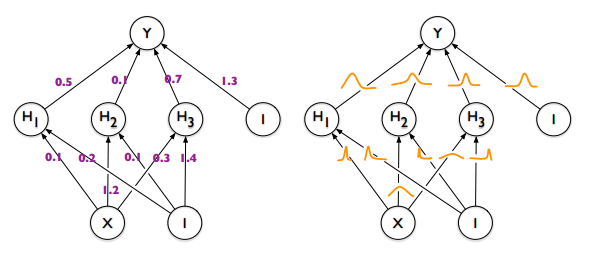
\includegraphics[width=0.75\linewidth]{assets/2-1.png}
    \caption{贝叶斯神经网络\cite{blundell2015weight}
}
    \label{fig:bnn}
\end{figure}


\begin{itemize}
    \item \textbf{贝叶斯推断}:
    通过贝叶斯公式来求解参数分布:
    \[
    P(\theta \mid \mathcal{D}) = \frac{P(\mathcal{D} \mid \theta) P(\theta)}{P(\mathcal{D})}
    \]
    其中:\( P(\theta \mid \mathcal{D}) \)是后验分布,\( P(\mathcal{D} \mid \theta) \)是似然函数,\( P(\theta) \)是先验分布, \( P(\mathcal{D}) \)是边际似然,用于归一化。

    
    \item \textbf{输出分布}:
    当输入图片到贝叶斯神经网络里预测时,输出的不是单一值,而是一个分布。从关于参数的后验分\( P(\theta \mid \mathcal{D}) \)采样多个 \( \theta \),通过这些 \( \theta \) 计算多个 \( y \),对 \( y \) 进行汇总(如计算熵或方差)得到不确定性。
\end{itemize}

贝叶斯神经网络的难题是后验分布 \( P(\theta \mid \mathcal{D}) \) 的估计。由于直接计算后验分布 \( P(\theta \mid \mathcal{D}) \) 通常是不可行的,贝叶斯神经网络采用近似方法,通常的近似手段有采样方法(如马尔科夫链蒙特卡罗方法)、变分推断、拉普拉斯近似等几种。马尔科夫链蒙特卡罗(MCMC)方法是一种通过随机抽样来逼近后验分布的方法。常见的 MCMC 算法包括 Metropolis-Hastings 算法和 Gibbs 采样。它们通过生成一系列样本来估计后验分布,但计算开销较大,尤其是在高维参数空间中。变分推断通过将后验分布近似为一个简单的分布族(例如高斯分布)来进行推断。它通过最小化某种距离度量(如 Kullback-Leibler 散度)来优化参数,使得近似分布尽可能接近真实的后验分布。拉普拉斯近似通过在后验分布的最大后验估计(MAP)附近用二次泰勒展开来近似后验分布。该方法对于参数空间较小或者后验分布接近高斯分布的情况特别有效。在使用贝叶斯神经网络建模不确定性的方法中,Charles Blundell\cite{blundell2015weight}等人提出了Bayes By Backprob算法高效地计算权重参数的后验分布。Yarin Gal\cite{gal2016dropout}从理论上证明Dropout可以用作深度高斯过程上贝叶斯推断的近似,进而提出MC Dropout量化模型的不确定性。这种方法在预测阶段保留 Dropout,并通过多次前向传播获得样本分布,该方法由于模型训练和预测都比较简单,成为广为采用的估计不确定性的思路。 Hippolyt Ritter\cite{ritter2018scalable}等人通过构建Kronecker分解的拉普拉斯近似,近似求解权重参数的后验分布。Welling等人\cite{welling2011bayesian}提出了一种称为 Stochastic Gradient Langevin Dynamics (SGLD) 的方法,结合了随机梯度下降 (SGD) 和 Langevin 动力学的思想,用随机梯度近似后验分布,同时引入噪声来模仿MCMC采样过程。



\subsection{模型集成方法}
在机器学习领域,集成(Ensemble)方法\cite{lakshminarayanan2017simple}\cite{fort2019deep}是一种通过训练多个模型并集成预测来提高性能和鲁棒性的技术。在建模不确定性时,集成方法的核心思想是通过多个独立模型的多样性来量化预测结果的可信度。集成方法通过训练多个独立的模型,每个模型从不同的角度对数据进行学习,并将这些模型的预测结果进行组合(例如取平均),可以提高整体的预测性能并提供不确定性估计。以下是模型集成方法的建模步骤:


\begin{enumerate}
    \item \textbf{训练多个模型}:
    训练 \( M \) 个独立的神经网络模型 \( f_1(x), f_2(x), \ldots, f_M(x) \),其中每个模型的参数初始化不同,或者使用不同的训练数据子集。

    \item \textbf{预测分布}:
    对于给定输入 \( x \),每个模型生成一个预测 \( y_i = f_i(x) \)。集成方法的预测分布可以通过这些独立模型的输出构造, 通过汇总预测分布的统计量(如方差、熵)来评估不确定性。
\end{enumerate}

模型集成方法建模不确定性理论比较简单且具有很好的不确定性建模效果,但是需要训练多个模型,计算和存储的复杂度比较高,如何减少模型集成方法存储和计算的复杂度是这一方法的难点。Y Wen\cite{wen2020batchensemble}等人提出BatchEnsemble解决模型集成方法需要训练多个模型的存储和计算复杂度,BatchEnsemble 将一个大模型分解为多个小模型,每个小模型具有自己的参数化方式,但它们共享同一个主干模型的参数。通过共享基础权重,BatchEnsemble 避免了传统模型集成方法中每个模型都需要独立存储全部参数的缺点。BatchEnsemble 大大减少了内存占用和计算需求。




\subsection{测试时数据增强的方法}
测试时数据增强(Test Time Agmentation,TTA)的方法是一种通过对测试数据应用多种数据增强方式来估计模型预测不确定性的方法。该方法通过将同一输入的不同增强版本的预测结果进行汇总,量化模型对该输入的不确定性,该方法的建模思路如下:


\begin{enumerate}
    \item \textbf{数据增强}:
    对测试数据 \( x \),应用一系列数据增强操作 \( T_1, T_2, \ldots, T_N \),生成多个增强版本 \( \{ T_i(x) \}_{i=1}^N \)。

    \item \textbf{预测分布}:
    对每个增强版本,模型 \( f \) 生成对应的预测结果 \( \{ f(T_i(x)) \}_{i=1}^N \)。通过汇总预测分布的统计量(如方差、熵)来评估不确定性。
\end{enumerate}

TTA建模不确定性只需要单个神经网络模型且很容易实现,但是存在的一个重要的问题是如何选择有效的数据增强方式。Divya Shanmugam等人\cite{shanmugam2020and}研究了如何选择合适的增强策略,以及在结果聚合(如简单平均、加权平均)中的设计方法。




\subsection{单一确定性神经网络建模}
由于传统的建模不确定性方法计算复杂度比较高,使用单一确定性的网络一次前向计算建模不确定性的方法是现阶段的研究热点,这也是本文研究的主要内容。单一确定神经网络建模不确定性,单一是指只需要训练一个神经网络,不像模型集成方法需要训练多个网络;确定是指网络参数是确定的,不像贝叶斯神经网络一样参数符合某个分布。这类方法建模不确定性通常直接从单一确定性模型的输出中直接推导出不确定性。这类方法通过模型结构或损失函数设计,使模型能够在不需要多模型或参数采样的情况下提供对不确定性的量化,从而降低计算和存储成本。单一确定神经网络可以分为内部性方法(Internal Methods)\cite{oala2020interval}和外部性方法(Externel Methods)\cite{gawlikowski2023survey}。

内部性方法是指不使用额外的头去预测不确定性,不确定性的计算和原有神经网络的预测是一起的。Internal Methods中,最先作为不确定性研究领域基线方法的是使用最大预测概率\cite{hendrycks2017a}(Maximum Softmax Probability, MSP)作为不确定性的度量。作者观察到,OOD 样本的MSP值通常会低于inD样本,因此可以使用MSP来建模不确定性。MSP简单易实现,直接利用现有神经网络的 Softmax 输出,无需修改网络架构或增加额外的训练开销,计算仅需一次前向传播,非常适合实时场景。Prior Network\cite{malinin2018predictive} 和DBU\cite{kopetzki2021evaluating}通过引入一个显式的先验分布来对分类问题中的不确定性建模。这种方法使用一个神经网络直接对分类器的分布进行建模,而不是仅输出点估计。Prior Network 的输出是一个分类概率分布的参数,例如 Dirichlet 分布的参数$\alpha$,用以表征预测的不确定性。Murat Sensoy等人\cite{sensoy2018evidential}提出了一个新方法,通过引入主观逻辑,在神经网络的分类概率上使用狄利克雷分布来量化不确定性。该方法将神经网络的分类结果视为主观意见,网络学习如何根据数据收集证据来支持每个类别的预测。这种方法不仅能预测分类结果,还能量化预测的不确定性,从而提升模型的鲁棒性。深度核学习(Deep Kernel Learning)\cite{van2021feature}结合深度神经网络和高斯过程,将神经网络的输出作为核函数的输入,捕捉数据的不确定性。

DUQ\cite{van2020uncertainty}通过使用与径向基函数(RBF)的结构,训练一个可以在推理时通过一次前向传播计算不确定性的模型。SNGP\cite{liu2020simple}核心思想是引入输入距离感知,即模型能够量化测试样本与训练数据之间的距离,从而准确评估预测的不确定性。论文提出了谱归一化神经高斯过程(SNGP),通过在训练中加入谱归一化\cite{yoshida2017spectral}步骤和替换倒数第二层的激活函数来增强模型的距离感知能力。DDU算法\cite{Mukhoti_2023_CVPR}通过高斯混合模型在神经网络提取的高维特征上构建一个高维概率分布,同时在训练时加上谱归一化,然后使用测试样本的高维特征在该分布上的概率密度建模神经网络的不确定性,DDU算法是本文研究对比的主要方法。

外部性方法显式地在原有模型基础上额外添加一个头来预测不确定性。Maithra Raghu等人\cite{raghu2019direct}提出了一种直接不确定性预测(Direct Uncertainty Prediction, DUP)方法,通过神经网络直接预测医学诊断任务中的预测置信度。由于不确定性标注的困难性,关于这类建模不确定性方法研究很少。




\subsection{以上主流方法的对比和分析}
下面对比以上列举的四类建模不确定性方法\ref{fig:uq}的优缺点。

贝叶斯神经网络(BNN)基于贝叶斯统计理论,具备良好的可解释性和数学基础,同时通过对网络参数进行概率建模,天然具有正则化效果。此外,在数据有限的情况下,先验分布能够提供有用的信息,从而提升模型性能。然而,BNN也面临诸多挑战,包括参数分布推断和采样的高计算复杂度、网络规模扩大后推断过程的难度增加,以及先验分布选择对模型性能的敏感性。

基于集成方法的不确定性建模通过组合多个模型的预测结果,有效降低了过拟合风险,提升了预测性能。无需修改模型结构,其方法能够灵活地与多种神经网络架构融合,并在多个代理任务中表现出卓越的不确定性建模能力。然而,集成方法的劣势也较为显著。训练多个模型需要大量计算资源和存储空间,尤其在深度学习场景下,开销尤为明显。此外,集成效果依赖子模型之间的多样性和质量,若模型过于相似,集成优势可能受到削弱。  

测试时数据增强(TTA)方法在不确定性建模中具有实现简便的特点。无需对模型结构或训练过程进行修改,仅通过测试阶段的增强技术即可实现建模。然而,TTA方法需要对同一输入进行多次推理,导致推理时间增加。此外,不同增强策略对不确定性估计的效果可能存在显著差异,因此策略设计需精心考量,以确保其有效性。  

\begin{figure}[H]
    \centering
    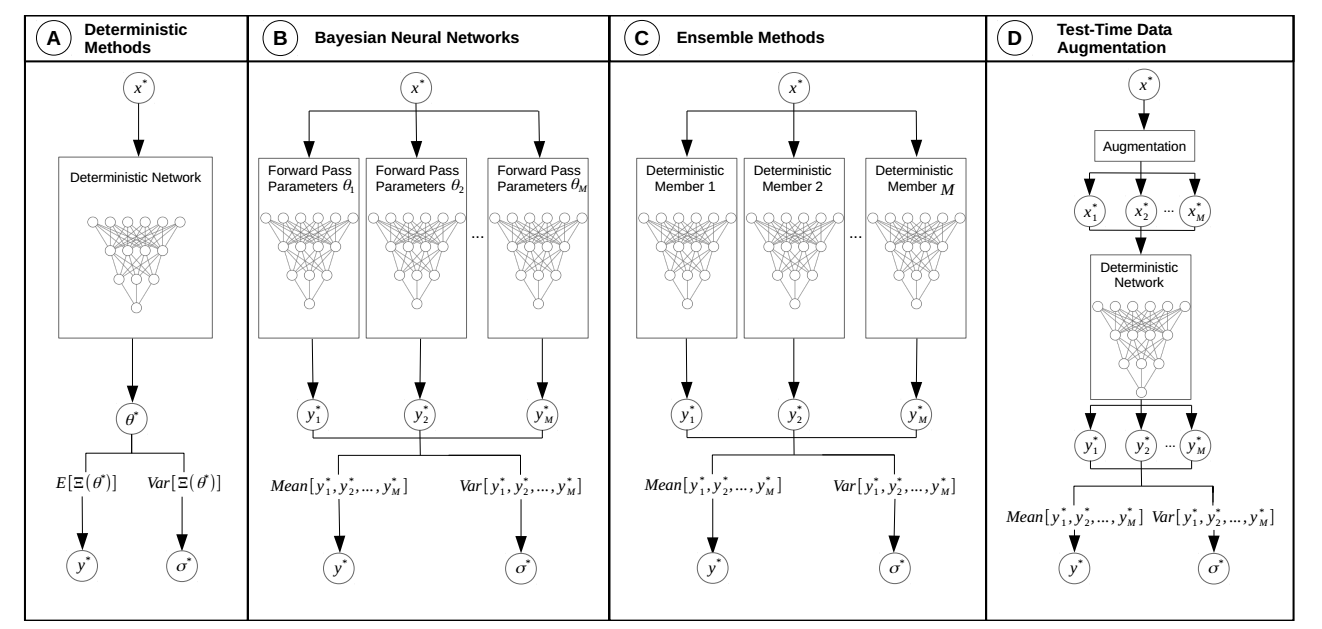
\includegraphics[width=0.9\linewidth]{assets/uq.png}
    \caption{主流的不确定性建模方法\cite{gawlikowski2023survey}
}
    \label{fig:uq}
\end{figure}

单一确定性网络则以高效性见长。通过设计合理的输出和损失函数即可实现不确定性建模,其推理速度快、计算成本低,且易于与现有神经网络框架结合。然而,相较于集成方法,单一确定性网络在建模效果上存在一定局限性,尤其当输出分布假设未能充分捕捉数据复杂分布时,可能导致不确定性估计不够精确。  

综上所述,当前主流不确定性建模方法通常依赖多次推理或模型集成,尽管效果出色,但计算复杂度较高。单一确定性网络提供了高效的替代方案,通过减少模型复杂性和推理开销,具备更大的应用潜力。本文旨在克服现有方法的局限性,基于高维特征的概率密度进行模型不确定性评估,并提出改进策略,以提升单一确定性网络的不确定性建模能力。

\section{不确定性的计算方法}
针对不同的建模不确定性的方法,对不确定性的计算方法各不相同,在分类任务上和回归任务上,对于不确定性的计算也不相同。以下列举几种常见情况下不确定性的计算公式。

\subsection{分类任务中不确定性的计算}

对于分类任务,模型输出每个类别的预测概率,模型的不确定性可以通过评估这些预测概率的分布来衡量,常见的计算方法包括最大概率\cite{hendrycks2017a}、熵\cite{wimmer2023quantifying}、互信息\cite{wimmer2023quantifying}等。

\textbf{最大概率}
    \[
    P_{\text{max}} = \max_{i} P(y_i | \mathbf{x})
    \]
    其中,\( P(y_i | \mathbf{x}) \) 是模型对样本 \( \mathbf{x} \) 的类别 \( y_i \) 的预测概率。最大概率 \( P_{\text{max}} \) 越接近1,表示模型的确定性越高;越接近0.5(对于二分类任务),表示不确定性较高。


\textbf{熵(Entropy)}:熵是衡量概率分布不确定性的标准方法。对于分类任务,熵的计算公式为:
\[
H(\mathbf{x}) = - \sum_{i=1}^{C} P(y_i | \mathbf{x}) \log P(y_i | \mathbf{x})
\]
其中,\( C \) 是类别数,\( P(y_i | \mathbf{x}) \) 是样本 \( \mathbf{x} \) 被预测为类别 \( y_i \) 的概率。熵越大,表示模型对样本的分类越不确定。


\textbf{互信息(Mutual Information)}:互信息衡量了输入特征与输出类别之间的信息共享量。在分类任务中,输入特征 \( \mathbf{x} \) 和输出类别 \( y \) 之间的互信息可以计算为:
\[
I(\mathbf{x}; y) = H(y) - H(y | \mathbf{x})
\]
其中,\( H(y) \) 是类别 \( y \) 的熵,表示输出的总体不确定性,\( H(y | \mathbf{x}) \) 是在给定输入 \( \mathbf{x} \) 的条件下,类别 \( y \) 的条件熵,表示输入特征给出的信息后,输出类别的剩余不确定性。互信息越大,表示输入特征与输出类别之间的关系越强,从而模型的预测不确定性越小。

\subsection{回归任务中不确定性的计算}
回归任务中,使用方差\cite{kendall2017uncertainties}、区间长度\cite{pearce2018high}等计算不确定性。

\textbf{方差}:对于回归任务,预测方差表示模型预测的不确定性。假设有多个模型的预测结果或多个预测实例,可以计算预测的方差:
\[
\text{Var}(\hat{y} | \mathbf{x}) = \frac{1}{T} \sum_{t=1}^{T} \left( y^{(t)} - \bar{y} \right)^2
\]
其中,\( \bar{y} = \frac{1}{T} \sum_{t=1}^{T} y^{(t)} \) 是预测值的均值,\( T \) 是预测次数。方差越大,模型预测的不确定性越高。

\textbf{区间长度}:预测区间表示模型预测值的上下限:
\[
[\hat{y} - \delta, \hat{y} + \delta]
\]
其中,\( \delta \) 是不确定性的度量(如标准差)。较大的 \( \delta \) 表示较高的不确定性。



\section{不确定性建模的评估}
近年来,随着不确定性建模方法的不断涌现,对这些方法的评估也显得尤为重要。由于大多数不确定性任务难以直接标注不确定性(即无法获得不确定性的标签),研究中普遍采用间接方式在代理任务上进行评估。常见的代理任务包括OOD 检测、误分类检测、对抗样本检测 和 主动学习。以下对每个任务如何评估不确定性进行具体介绍。

\subsection{OOD 检测}

OOD检测(Out-of-Distribution Detection) 任务的目标是在测试过程中识别出那些来自训练集分布外的样本。OOD 样本通常与训练数据的分布显著不同。理想情况下,好的不确定性建模方法应该对 OOD 样本表现出高不确定性。在使用OOD检测任务评估不确定性建模方法的过程中,使用来自训练分布的数据集作为正样本(In-Distribution, InD),来自训练集分布外的数据集的样本作为 OOD 样本,对OOD样本和InD样本分别计算不确定性,如果计算出来的不确定性对于OOD样本和InD样本区分性比较好,那么这种不确定性建模方法就是更好的。从这个角度上来看,不确定性建模的好坏和OOD检测任务是统一的。为了度量计算出的不确定性在区分OOD样本和InD样本的好坏,通常使用机器学习中AUROC,AUPRC等指标。

AUROC(Area Under the Receiver Operating Characteristic Curve,接收者操作特征曲线下面积),是一种衡量二分类模型性能的指标。在二分类任务中,混淆矩阵(Confusion Matrix)是评估分类模型性能的一个重要工具,其定义如表\ref{confusion}:
\begin{table}[H]
\centering
\begin{tabular}{|c|c|c|}
\hline
 & \textbf{预测为正类}  & \textbf{预测为负类}  \\
\hline
\textbf{实际为正类}  & TP (True Positive) & FN (False Negative) \\
\hline
\textbf{实际为负类} & FP (False Positive) & TN (True Negative) \\
\hline
\end{tabular}
\caption{二分类任务中的混淆矩阵 (Confusion Matrix)}
\label{confusion}
\end{table}

根据以上混淆矩阵,真阳性率 (True Positive Rate, TPR)和假阳性率 (False Positive Rate, FPR)计算公式如下:
\[
\text{TPR} = \frac{\text{TP}}{\text{TP} + \text{FN}}
\]

\[
\text{FPR} = \frac{\text{FP}}{\text{FP} + \text{TN}}
\]

ROC 曲线是通过改变分类阈值来绘制的,横轴为 FPR,纵轴为 TPR。AUROC 是 ROC 曲线下的面积,当 \(\text{AUROC} = 0.5\) 时,模型没有任何区分能力,表现与随机猜测相同。当 \(\text{AUROC} = 1.0\) 时,模型能够完美区分正负类。当 \(0.5 < \text{AUROC} < 1.0\) 时,模型具有一定的区分能力,值越大表示性能越好。AUROC 是一个不依赖于特定分类阈值的评估指标,尤其适合于不平衡数据集的情况。

AUPRC(Area Under the Precision-Recall Curve,精确率-召回率曲线下面积)是评估分类模型性能的另一个常用指标,表示精度-召回率曲线下的面积。根据混淆矩阵,精度 (Precision)和召回率 (Recall)计算公式如下:

\[
\text{Precision} = \frac{\text{TP}}{\text{TP} + \text{FP}}
\]


\[
\text{Recall} = \frac{\text{TP}}{\text{TP} + \text{FN}}
\]



Precision-Recall曲线展示了不同分类阈值下的精度与召回率之间的关系。AUPRC 是该曲线下的面积。当 \(\text{AUPRC} = 0\) 时,模型完全没有区分能力。当 \(\text{AUPRC} = 1.0\) 时,模型在所有召回率下的精度都为 1,表示模型完美区分正负类。
当 \(0 < \text{AUPRC} < 1.0\) 时,模型具有一定的区分能力,AUPRC 值越大表示性能越好。AUPRC 尤其适用于不平衡数据集的情况,因为它直接衡量了在正类样本较少时的分类性能。




\subsection{误分类样本识别}


误分类样本识别的目标是利用对预测结果计算出的不确定性信息识别模型预测错误的样本。理想情况下,模型应对误分类样本表现出高不确定性。使用误分类检测作为代理任务,通过分析模型在测试数据上的误分类样本,观察不确定性分布是否能有效区分正确分类与错误分类的样本,判断不确定性建模算法的好坏。除了包括与OOD 检测类似的常用指标AUROC 和 AUPRC。还有Expected Calibration Error (ECE)\cite{guo2017calibration},衡量模型预测置信度与实际准确率的偏差。Expected Calibration Error (ECE) 是衡量分类模型输出概率与实际标签一致性的一个指标。一个校准良好的模型,其预测概率应当与实际结果的发生频率一致。具体地,若模型预测概率为 \( p \),那么在长期实验中,模型预测为 \( p \) 的样本中,有 \( p \) 的比例应该属于正类。下面是ECE的计算方法:


1. 分组:
   将预测概率 \( p \) 分成若干个区间,例如: [0, 0.1), [0.1, 0.2), \dots, [0.9, 1.0] 这些区间可以根据需要调整。

2. 计算每个区间的校准误差:
   对于第 \( k \) 个区间 \( [p_k, p_{k+1}) \),计算该区间内所有样本的平均预测概率 \( \hat{p}_k \) 和真实标签的正确率 \( \text{accuracy}_k \)
   % \[
   % \hat{p}_k = \frac{1}{|S_k|} \sum_{i \in S_k} p_i
   % \]
   % \[
   % \text{accuracy}_k = \frac{1}{|S_k|} \sum_{i \in S_k} y_i
   % \]
   % 其中,\( S_k \) 是属于第 \( k \) 个区间的样本集合,\( p_i \) 是样本 \( i \) 的预测概率,\( y_i \) 是样本 \( i \) 的真实标签。

3. 计算校准误差:对每个区间计算校准误差,并计算所有区间的加权平均值:
\[
   \text{ECE} = \sum_k \frac{|S_k|}{N} | \hat{p}_k - \text{accuracy}_k |
   \]
   其中,\( N \) 是样本总数,\( |S_k| \) 是第 \( k \) 区间内样本的数量。


当 \(\text{ECE} = 0\) 时,表示模型是完全校准的,预测概率与实际频率完全一致。当 \(\text{ECE}\) 较大时,表示模型存在较大的校准误差,其概率输出与实际标签的匹配不佳。





\subsection{对抗样本检测}

对抗样本(Adversarial Examples) 是指通过对输入数据添加精细、刻意设计的微小扰动,使得机器学习模型对这些输入产生误判的样本。这些扰动通常对人类来说是不可察觉的,但会显著影响模型的预测结果。对抗样本检测的目标是识别经过精心设计以欺骗模型的样本。理想情况下,模型对对抗样本的预测应表现出更高的不确定性,所以使用不确定性作为对抗样本检测的指标,对抗样本识别的效果越好,不确定性建模的效果越好。对抗样本检测作为代理任务,评估不确定性建模方法好坏的思路是:首先使用一定的攻击算法生成一批对抗样本(如 FGSM\cite{goodfellow2015explaining} 、BIM\cite{kurakin2016adversarial}、PGD\cite{madry2017towards} 攻击),然后与正常样本一起输入模型并计算不确定性,检测不确定性是否能区分对抗样本与正常样本。衡量指标与 OOD 检测相同,主要使用 AUROC 和 AUPRC 来评估,AUROC和AUPRC两个指标越高,说明不确定性建模的效果越好。


\subsection{主动学习}


主动学习(Active Learning)\cite{ren2021survey}\cite{settles2009active}是一种机器学习方法,其中模型通过选择最具信息量的样本进行标注,以便在最少的标注成本下获得最大的学习效果。与传统的监督学习不同,主动学习不依赖于全部标注数据,而是通过一个学习算法主动选择样本,从而最大化模型的性能。一般的主动学习流程见\ref{fig:al}
\begin{figure}[h]
    \captionsetup{font=small, justification=centering}
    \centering
    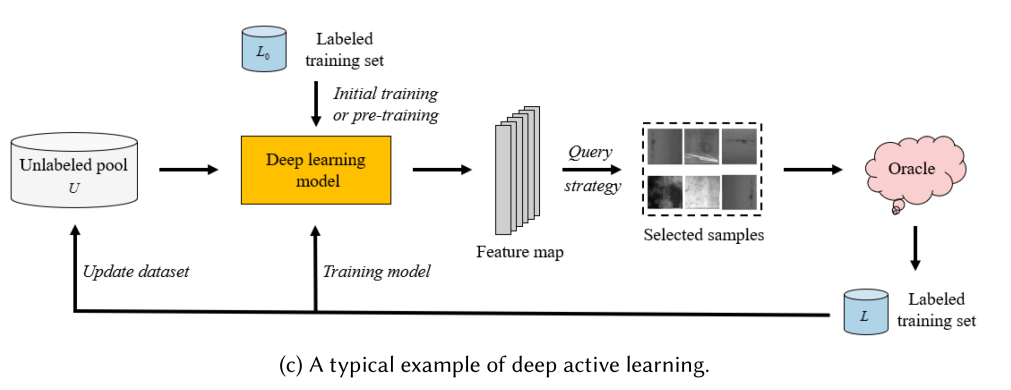
\includegraphics[width=0.9\linewidth]{assets/activelearning.png}
    \caption{主动学习一般的流程\cite{ren2021survey}}
    \label{fig:al}
\end{figure}

在有限标注预算下,主动学习通过选择具有高不确定性的样本来优化标注数据集的选择策略。一个好的不确定性建模方法应能快速有效挑选提升模型性能的样本。通过迭代方式模拟主动学习过程,每轮根据不确定性选择样本进行标注,在固定训练样本规模下,通过主动学习策略挑选的样本训练模型,观察训练后的性能提升,如果依照不确定性挑选的样本能以较少标注样本达到目标性能,这种不确定性建模方法是良好的。主动学习评估不确定性建模方法的基本工作流程如下:

\begin{enumerate}[nosep]
    \item \textbf{初始化数据集}:首先从未标注的数据池中随机选择一小部分样本,并对这些样本进行标注,构成初始训练集。
    \item \textbf{模型训练}:使用初始训练集训练模型。
    \item \textbf{选择样本}:根据模型的当前性能,从未标注数据池中选择最能提高模型性能的样本。选择策略是依据不确定性采样,从候选池中选择模型最不确定的样本进行标注。
    \item \textbf{标注和迭代}:对选择的样本进行标注,加入到训练集中,然后重新训练模型。重复选择样本和训练的过程,直到满足某个停止条件(例如,达到一定的精度或标注次数)。
\end{enumerate}

\section{本章小结}
本章主要围绕不确定性的研究工作与理论展开讨论,分别从不确定性的建模方法、计算方法以及评估方法三个角度进行阐述。首先,介绍了几类主流的不确定性建模方法,包括贝叶斯神经网络、集成方法、测试时数据增强方法以及单一确定性神经网络建模,并详细对比了它们在优缺点。其次,本章介绍了分类与回归任务中不确定性计算的具体方式,例如分类任务中基于Softmax输出的预测熵、互信息和回归任务中的方差及预测区间长度等。最后指出由于标签信息的缺乏,模型的不确定性评估多依赖代理任务的表现,而非直接评估方法。整章通过分析总结不确定性建模领域的重要研究进展与挑战,为后续工作奠定了理论基础。

